%subsection
\begin{comment}
IoTサービスの開発と運用における要件を引き出すために、岡本商店街での実験を行った。
・実験の概要
・開発したサービスの説明
・用いた機器や開発したプログラム等の説明
 ・どのように開発したのか
\end{comment}

\subsubsection{実験概要}
2015年12月8日から2016年2月26日まで、NPO法人コミュニティリンクへのインターンシップの一環として、岡本商店街にて人流観測実験を行った。
岡本商店街とは、神戸市東灘区にある阪急岡本駅とJR摂津本山駅の間にある商店街のことである。
実験は、IoTに関連する技術を用い人流観測を行い、結果を分析し商店街の活性化に役立てるという趣旨で行った。
観測は、2016年2月7日から2016年3月14日まで行った。

人流観測とは、各地点から各地点迄をある時に移動した人数を観測するものである。
通常は、観察員がカウンタを用いて数えるが、それでは各地点間を移動した人数はわかるが、その人が以前どの地点に居たのかはわからない。
そこで、携帯電話についているWifi機能を利用し、観測を行うこととした。
携帯電話のWifi機能は、無線LANの接続に使われるが、接続毎にWifi機能を有効にすることが手間なため、常時ONにしている人も少なくない。
携帯電話のWifi機能を有効にしている場合、携帯電話から接続可能な無線LANを探す為、プローブパケットというものが定期的に送出される。
プローブパケットには、そのプローブパケットを送出した機器の物理アドレスが含まれており、個々の機器が識別可能である。
そのプローブパケットを複数地点で観測し、含まれている物理アドレスと受信時刻を照合することで、携帯電話端末を持った人がどのように移動をしたのかが分かる。
岡本商店街では、この原理を利用して、人流観測を行った。

\subsubsection{観測・分析・可視化システムの構成}
本事例では、岡本商店街の5店舗に開発した観測機器を設置し、サーバにて蓄積・分析・可視化を行った。
構成としては、観測機器内で動作するプログラムが定期的にサーバーに観測データを送信する。
サーバ上では、分析プログラムと可視化プログラムが動作しており、観測データは分析プログラムへ渡される。
分析プログラムは、観測データを可視化プログラムの要求によって分析し、結果を可視化プログラムへ渡す。
可視化プログラムは、ユーザからの操作によって分析プログラムを呼び出し、分析結果をWebインターフェースによって可視化する。
このシステムのユーザーは、ブラウザからWebインターフェースへアクセスすることで、操作・分析結果の閲覧をすることができる。
図\ref{fig:okamoto_diag1}は、開発したシステムの構成を示している。
\begin{figure}[htbp]
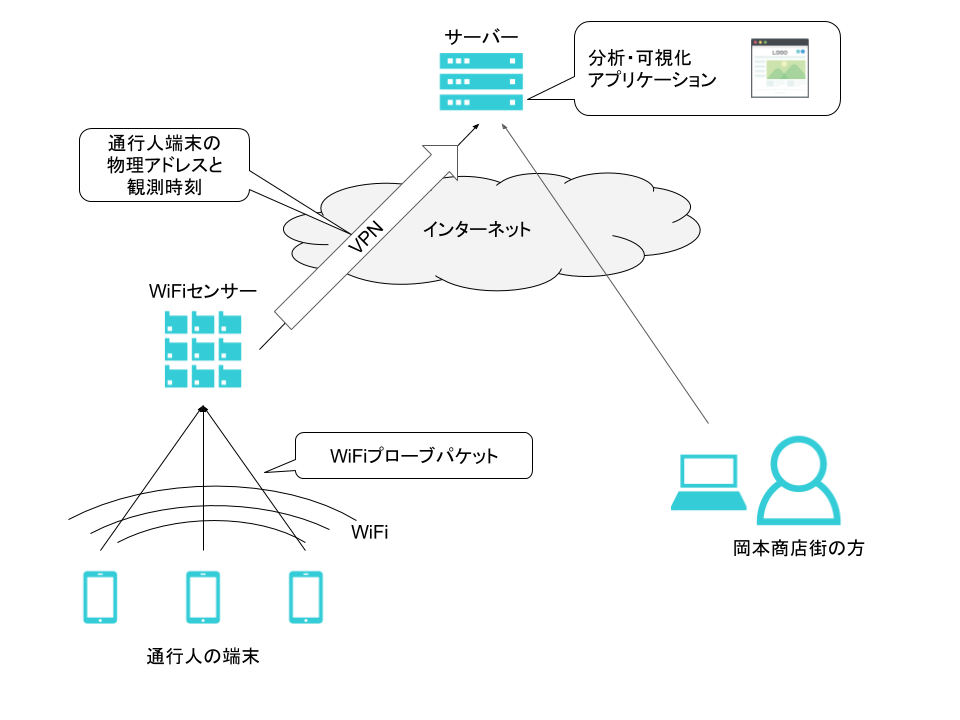
\includegraphics[width=16cm]{images/okamoto_diag1.png}
\caption{岡本商店街人流観測 構成図}
\label{fig:okamoto_diag1}
\end{figure}

開発した観測機器は、RaspberryPiとBaffalo製のWifiドングル、ampsence・rsyncというソフトウェアを利用し作成した。
図\ref{fig:okamoto_pict1}は、開発した観測機器である。
\begin{figure}[htbp]
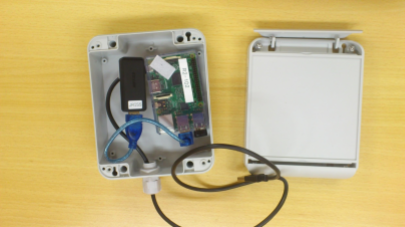
\includegraphics[width=16cm]{images/okamoto_pict1.png}
\caption{岡本商店街人流観測 使用した機器}
\label{fig:okamoto_pict1}
\end{figure}
RaspberryPiとは、小型PCの一つで安価に入手が可能である。
また、利用したRaspberryPiにはWifiインターフェースが存在しなかったので、Baffalo製のUSB接続が可能なWifiドングルを接続した。
ampsenceとは、プローブパケットを受信しプローブパケットに含まれる物理アドレスと観測日時をファイルへ記録するソフトウェアである。
rsyncとは、ディレクトリの中を同期させるプログラムで、遠隔にあるコンピュータの指定したディレクトリの中と、手元のコンピュータの指定したディレクトリを同期することができる。
開発した観測機器は、起動時にampsenceを動作させ、定期的にrsyncを実行するよう設定した。
これによって、各所に設置された観測機器の情報をサーバー上に集約・蓄積する。

作成した分析プログラムは、可視化プログラムから指定された期間内の観測データを読み込み、地点ごと観測時間ごとの物理アドレスの数の推移・地点ごと観測時間ごとの移動した人数の割合を集計し、可視化プログラムへ渡す。
作成した可視化プログラムは、ユーザから指定された期間を分析プログラムへ渡し、分析結果を棒グラフや円グラフといった形で、ユーザーへ表示する。
図\ref{fig:okamoto_ss}は作成したWebアプリケーションである。
\begin{figure}[htbp]
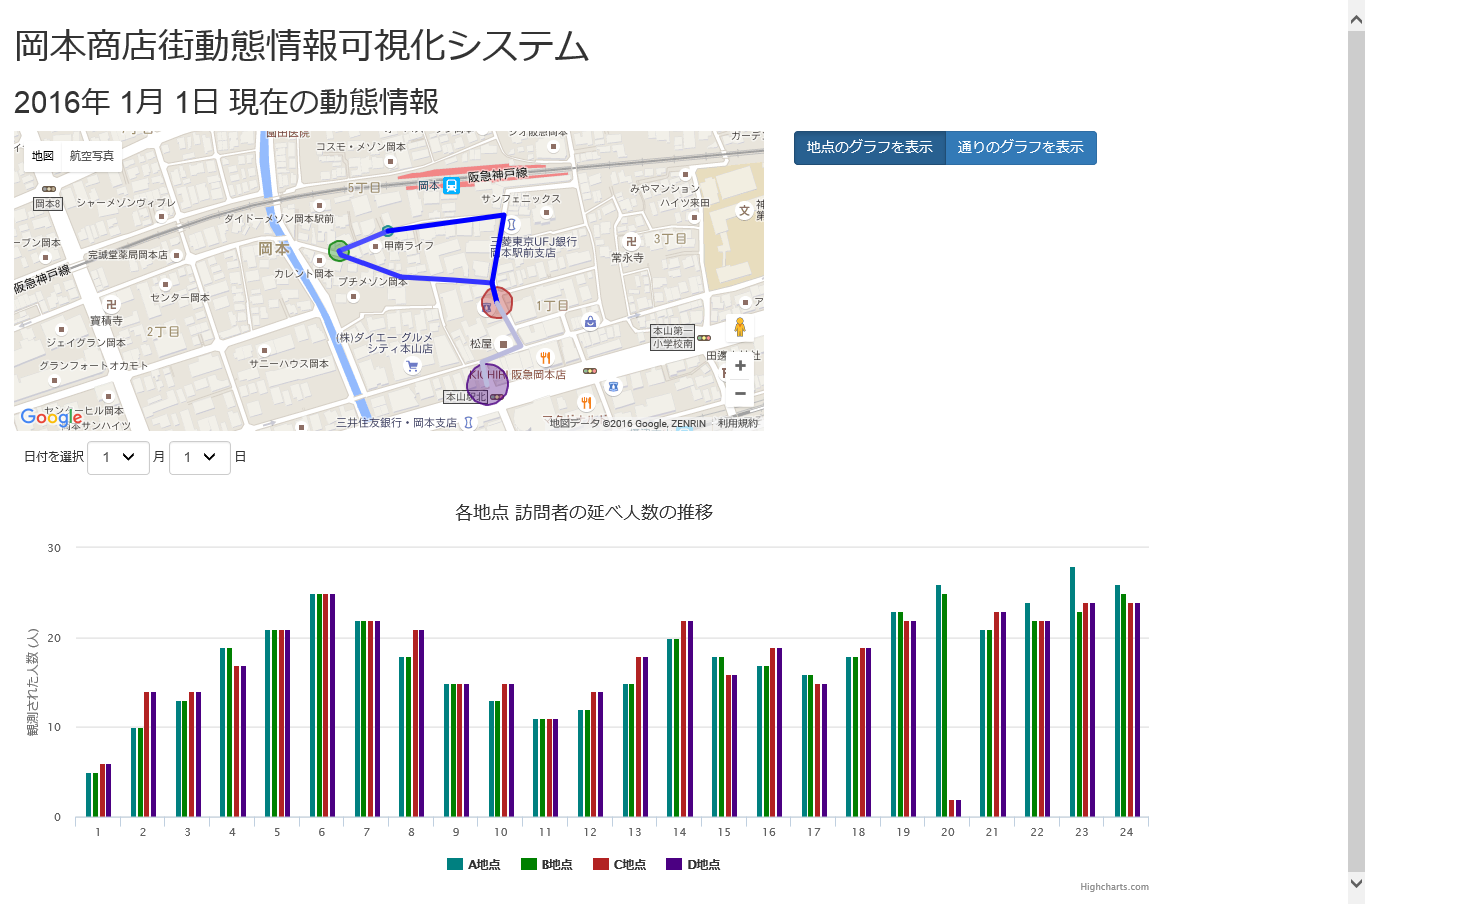
\includegraphics[width=16cm]{images/okamoto_scr1.png}
\caption{岡本商店街人流観測可視化アプリケーションスクリーンショット}
\label{fig:okamoto_ss}
\end{figure}

\subsection{実験にあたって考慮した点}
実験機材の開発と実験を行うにあたって、次のような点を考慮し、作成した。
\begin{itemize}
\item 機器が設置されるネットワークは、店舗のネットワークであるため、ネットワーク機器の設定等を変更せずに設置することができるよう考慮した。
\item ソフトウェアのアップデートやトラブルに備え、VPNを張り、VPN越しにログインできるように設定した。
\item 店舗ネットワークが利用できない個所の場合は、SORACOM Airを用いることとした。
\item サーバー側の不良に備え、機器自体にも情報を蓄積しておくことにした。
\end{itemize}

\subsection{実験結果}
実験によって、次のような結果が得られた。


\subsection{実験でのトラブル}
しかし、実験の際に次のような点が問題となった。


\subsection{考察}













\begin{comment}
どうしたら良いのかわからなくなっている。

頭の中では、このようなストーリーかなと考えている。
1.岡本商店街でこんなことをやった
 1.こんな人流観測をしました。
  1.岡本商店街とは
  2.人流観測とは
  3.こんなものを使って観測しました。
  4.こんな結果が得られました。
 2.だけど、機器の監視が大変でした。それによってこんな問題がおきました。
  1.こんなトラブルが有りました。
  2.それによってこんな問題がありました。
  3.なので、監視が必要と思いました。
2.何故大変だったのか、考えてみました。
 1.まず、岡本商店街での問題を整理しました。
  1.機器の数が多いことで、こんな問題が有りました。
  2.機器が接続するネットワークにNAPTがあったので、このように困りました。
 2.他の人達はこのことについてどう思っているのか聞いてみました。
  1.ルナネクサスさんへヒアリング
  2.SORACOMさんへヒアリング
  3.以上2件から、皆機器の監視について困っていることがわかりました。
3.ヒアリングの結果を元に、こんな物が有れば良いのではと思いました。
 1.機器がNAPTの内側にあっても、動いているのか監視できる事が必要だと思いました。
 2.ネットワークが違っていても、同じUIで閲覧できる事が必要だと思いました。
 3.機器を追加する時に、あまり手間がかからないことも大切だと思いました。
 4.セキュリティの都合でブロックされることが無い事も大切だと思いました。
4.作ってみました
 1.システムの全体像(こんな感じの物をつくってみました)
 2.各要素の説明(各要素はこんな動きをします)
 3.各要素の関連(各要素同士はこんなふうに連携します)
5.役に立ったか検証してみました
 1. 必要となる機能が満たされているかどうか検証してみました。
  1.機器の現在の状態の確認ができる事を確認しました。
  2.機器の過去の状態が確認できることを確認しました。
 2. 実際に役に立ったのか検証してみました。
  1.時間がなかった事と、使ってくれるユーザーがいなかったので検証できませんでした。
\end{comment}








